\documentclass[DIN, pagenumber=false, fontsize=11pt, parskip=half]{scrartcl}
\usepackage[UTF8]{ctex}  % 中文支持
% \usepackage{ngerman}
\usepackage[utf8]{inputenc}
\usepackage[T1]{fontenc}
\usepackage{textcomp}
\usepackage{xcolor} % Required for custom red

\usepackage{geometry} % Custom margins

\usepackage{tocloft} % Modifying the table of contents

% for matlab code
% bw = blackwhite - optimized for print, otherwise source is colored
\usepackage[framed,numbered,bw]{mcode}
\usepackage[most]{tcolorbox}
% for other code
%\usepackage{listings}
\usepackage{pgfplots}
\pgfplotsset{compat=1.15}
\usepackage{mathrsfs}
\usetikzlibrary{arrows}
\pagestyle{empty}
 

%<<<<<<<WARNING>>>>>>>
% PGF/Tikz doesn't support hatch filling very well
% Use PStricks for a perfect hatching export

\usetikzlibrary[patterns]

\setlength{\parindent}{0em}

% set section in CM
\setkomafont{section}{\normalfont\bfseries\Large}

\newcommand{\mytitle}[1]{{\noindent\Large\textbf{#1}}}
\newcommand{\mysection}[1]{\textbf{\section*{#1}}}
\newcommand{\mysubsection}[2]{\romannumeral #1) #2}

\newtcolorbox{parchmentquote}{
    enhanced,
    colback=orange!5!white,   % 浅米黄色背景
    colframe=orange!50!black,
    boxrule=0.5pt,
    arc=2pt,                  % 细微圆角
    boxsep=5pt,
    before skip=10pt,
    after skip=10pt,
    fontupper=\itshape,
    borderline west={2pt}{0pt}{orange!80!black} % 加厚的左装饰线
}
%===================================
\begin{document}

\noindent\textbf{课下讲义} \hfill \textbf{face-to-face course}\\
primary school \hfill Liu\\

\mytitle{期中小结 \hfill \today}
\newline
\begin{parchmentquote}
    复杂图形的周长是有做题方法的，但是不管怎样，基础放在第一位。
\end{parchmentquote}


%===================================
\section{图形周长的认识}
周长是指环绕有限区域的\textbf{封闭边界}的总长度
\newline
如图所示，只有外部的边界一周才是周长，内部$GD$的长度不算在周长内。
% \begin{tikzpicture}
%     % 画长方形
%     \draw[thick] (0,0) rectangle (5,3);

%     % 添加长度标注
%     % mid-way 自动找到线段中点，below/left 设置文字方位
%     % \draw[<->] (0,-0.3) ;
%     % \draw[<->] (-0.3,0) -- node[left] {$b = 3\,\text{cm}$} (-0.3,3);

%     % 在中心标注面积

% \end{tikzpicture}
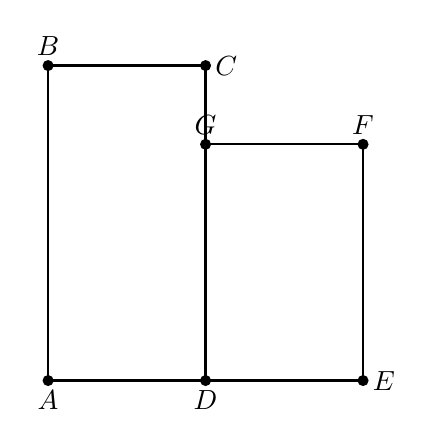
\begin{tikzpicture}
    % 定义点变量 A 和 B
    \coordinate (A) at (0,0);
    \coordinate (B) at (0,4);
    \coordinate (C) at (2,4);
    \coordinate (D) at (2,0);
    \coordinate (E) at (4,0);
    \coordinate (F) at (4,3);
    \coordinate (G) at (2,3);

    % 使用变量连线
    \draw[thick] (A) -- (B);
    \draw[thick] (B) -- (C);
    \draw[thick] (C) -- (D);
    \draw[thick] (D) -- (E);
    \draw[thick] (E) -- (F);
    \draw[thick] (F) -- (G);
    \draw[thick] (A) -- (D);

    % 计算并标记中点 M (需要加载 calc 库)
    % \usetikzlibrary{calc}


    % 绘制点并标注文字
    \fill (A) circle (2pt) node[below] {$A$};
    \fill (B) circle (2pt) node[above] {$B$};
    \fill (C) circle (2pt) node[right] {$C$};
    \fill (D) circle (2pt) node[below] {$D$};
    \fill (E) circle (2pt) node[right] {$E$};
    \fill (F) circle (2pt) node[above] {$F$};
    \fill (G) circle (2pt) node[above] {$G$};

\end{tikzpicture}
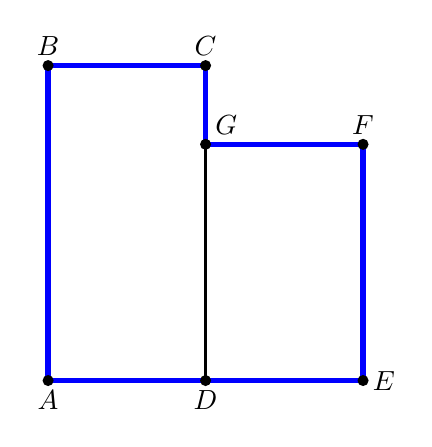
\begin{tikzpicture}
    % 定义点变量 A 和 B
    \coordinate (A) at (0,0);
    \coordinate (B) at (0,4);
    \coordinate (C) at (2,4);
    \coordinate (D) at (2,0);
    \coordinate (E) at (4,0);
    \coordinate (F) at (4,3);
    \coordinate (G) at (2,3);

    % 使用变量连线
    \draw[blue,line width=2pt ] (A) -- (B);
    \draw[blue,line width=2pt] (B) -- (C);
    \draw[thick] (C) -- (D);
    \draw[thick] (D) -- (E);
    \draw[blue,line width=2pt] (E) -- (F);
    \draw[blue,line width=2pt] (F) -- (G);
    \draw[thick] (A) -- (D);
    \draw[blue,line width=2pt] (A) -- (E);
    \draw[blue,line width=2pt] (C) -- (G);

    % 计算并标记中点 M (需要加载 calc 库)
    % \usetikzlibrary{calc}


    % 绘制点并标注文字
    \fill (A) circle (2pt) node[below] {$A$};
    \fill (B) circle (2pt) node[above] {$B$};
    \fill (C) circle (2pt) node[above] {$C$};
    \fill (D) circle (2pt) node[below] {$D$};
    \fill (E) circle (2pt) node[right] {$E$};
    \fill (F) circle (2pt) node[above] {$F$};
    \fill (G) circle (2pt) node[above right] {$G$};

\end{tikzpicture}
\section{几种常见的图形}
\subsection{篱笆问题}
\begin{center}
    \begin{figure}[htbp]
        \centering
        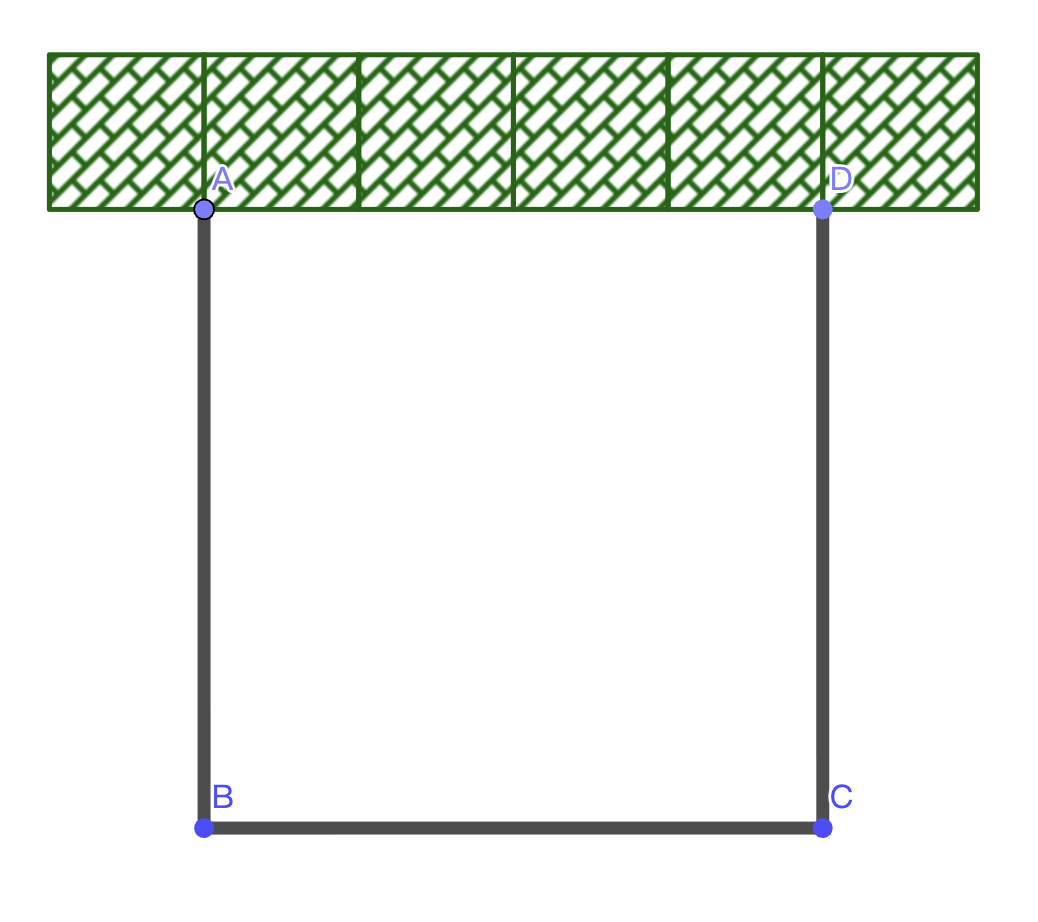
\includegraphics[width=0.2\textwidth]{liba_2.png}
        \caption{截图}
        \label{fig:example}
    \end{figure}
\end{center}

\subsection{缺一角的长方形}
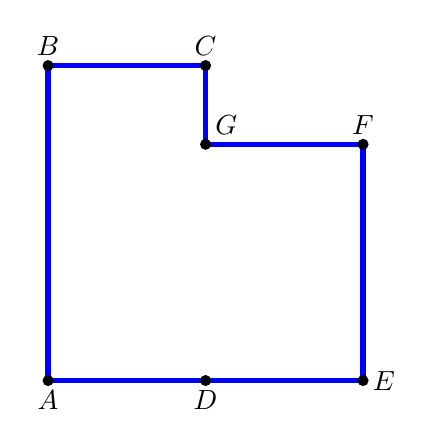
\begin{tikzpicture}
    % 定义点变量 A 和 B
    \coordinate (A) at (0,0);
    \coordinate (B) at (0,4);
    \coordinate (C) at (2,4);
    \coordinate (D) at (2,0);
    \coordinate (E) at (4,0);
    \coordinate (F) at (4,3);
    \coordinate (G) at (2,3);
    \coordinate (H) at (2,3);

    % 使用变量连线
    \draw[blue,line width=2pt ] (A) -- (B);
    \draw[blue,line width=2pt] (B) -- (C);
    \draw[thick] (C) -- (G);
    \draw[thick] (D) -- (E);
    \draw[blue,line width=2pt] (E) -- (F);
    \draw[blue,line width=2pt] (F) -- (G);
    \draw[thick] (A) -- (D);
    \draw[blue,line width=2pt] (A) -- (E);
    \draw[blue,line width=2pt] (C) -- (G);

    % 计算并标记中点 M (需要加载 calc 库)
    % \usetikzlibrary{calc}


    % 绘制点并标注文字
    \fill (A) circle (2pt) node[below] {$A$};
    \fill (B) circle (2pt) node[above] {$B$};
    \fill (C) circle (2pt) node[above] {$C$};
    \fill (D) circle (2pt) node[below] {$D$};
    \fill (E) circle (2pt) node[right] {$E$};
    \fill (F) circle (2pt) node[above] {$F$};
    \fill (G) circle (2pt) node[above right] {$G$};

\end{tikzpicture}
\newline
周长与缺失的角无关，仍然是$2\times(AB+AE)$。

\subsection{中间挖去一个长方形}
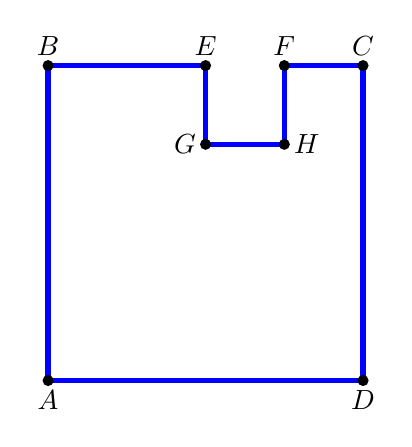
\begin{tikzpicture}
    % 定义点变量 A 和 B
    \coordinate (A) at (0,0);
    \coordinate (B) at (0,4);


    \coordinate (D) at (4,0);
    \coordinate (C) at (4,4);
    \coordinate (E) at (2,4);
    \coordinate (F) at (3,4);
    \coordinate (G) at (2,3);
    \coordinate (H) at (3,3);


    % 使用变量连线
    \draw[blue,line width=2pt ] (A) -- (B);
    \draw[blue,line width=2pt] (B) -- (E);
    \draw[blue,line width=2pt] (E) -- (G);
    \draw[blue,line width=2pt] (G) -- (H);
    \draw[blue,line width=2pt] (H) -- (F);
    \draw[blue,line width=2pt] (F) -- (C);
    \draw[blue,line width=2pt] (C) -- (D);
    \draw[blue,line width=2pt] (D) -- (A);



    % 计算并标记中点 M (需要加载 calc 库)
    % \usetikzlibrary{calc}


    % 绘制点并标注文字
    \fill (A) circle (2pt) node[below] {$A$};
    \fill (B) circle (2pt) node[above] {$B$};
    \fill (C) circle (2pt) node[above] {$C$};
    \fill (D) circle (2pt) node[below] {$D$};
    \fill (E) circle (2pt) node[above] {$E$};
    \fill (F) circle (2pt) node[above] {$F$};
    \fill (G) circle (2pt) node[left] {$G$};
    \fill (H) circle (2pt) node[right] {$H$};


\end{tikzpicture}
\newline
周长比以前的长方形增加了$EG+FH$。

\subsection{一个练习}
把一个长14厘米的长方形剪成6个大小相同的小长方形，这6个小长方形的周长比原来的长方形的周长增加64厘米，这个大长方形的宽是多少厘米？
\newline
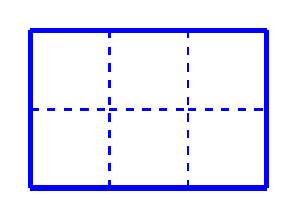
\begin{tikzpicture}
    % 定义点变量 A 和 B
    \coordinate (A) at (0,0);
    \coordinate (B) at (1,0);
    \coordinate (C) at (2,0);
    \coordinate (D) at (3,0);
    \coordinate (E) at (0,1);
    \coordinate (F) at (1,1);
    \coordinate (G) at (2,1);
    \coordinate (H) at (3,1);
    \coordinate (I) at (0,2);
    \coordinate (J) at (1,2);
    \coordinate (K) at (2,2);
    \coordinate (L) at (3,2);



   


    % 使用变量连线
    \draw[blue,line width=2pt ] (A) -- (B);
    \draw[blue,line width=2pt] (B) -- (C);
    \draw[blue,line width=2pt] (C) -- (D);
    \draw[blue,line  width=2pt] (A) -- (E);
    \draw[blue,dashed,line width=1pt] (E) -- (F);
    \draw[blue,dashed,line width=1pt] (F) -- (G);
    \draw[blue,dashed,line width=1pt] (G) -- (H);
    \draw[blue,dashed,line width=1pt] (B) -- (J);
    \draw[blue,dashed,line width=1pt] (C) -- (K);
      \draw[blue,line  width=2pt] (E) -- (I);
      \draw[blue,line  width=2pt] (I) -- (J);
      \draw[blue,line  width=2pt] (J) -- (K);
      \draw[blue,line  width=2pt] (K) -- (L);
      \draw[blue,line  width=2pt] (D) -- (H);
      \draw[blue,line  width=2pt] (H) -- (L);
    \draw[blue,line width=2pt] (D) -- (A);

\end{tikzpicture}


\section{除数小结}
两数相除商8余7，被除数、除数、商和余数四个数的和是103，被除数与除数各是多少？
被除数$ \div $除数 = 商 $\ldots$ 余数 \newline
被除数$ \div $除数 = $8 \ldots 7$
\section{其他问题}
\begin{enumerate}
    \item 长方形与正方形的周长、面积公式牢记
    \item 计算题不要出错
    \item 复杂图形的周长要画图，标出已知边，找出缺失边，最后计算周长。
    \item 对称轴这个不难，但是全部找出还是要花心思
\end{enumerate}

\end{document}